
\section{Hardware}
\label{section_Hardware}

\begin{figure}[H]
\begin{center}
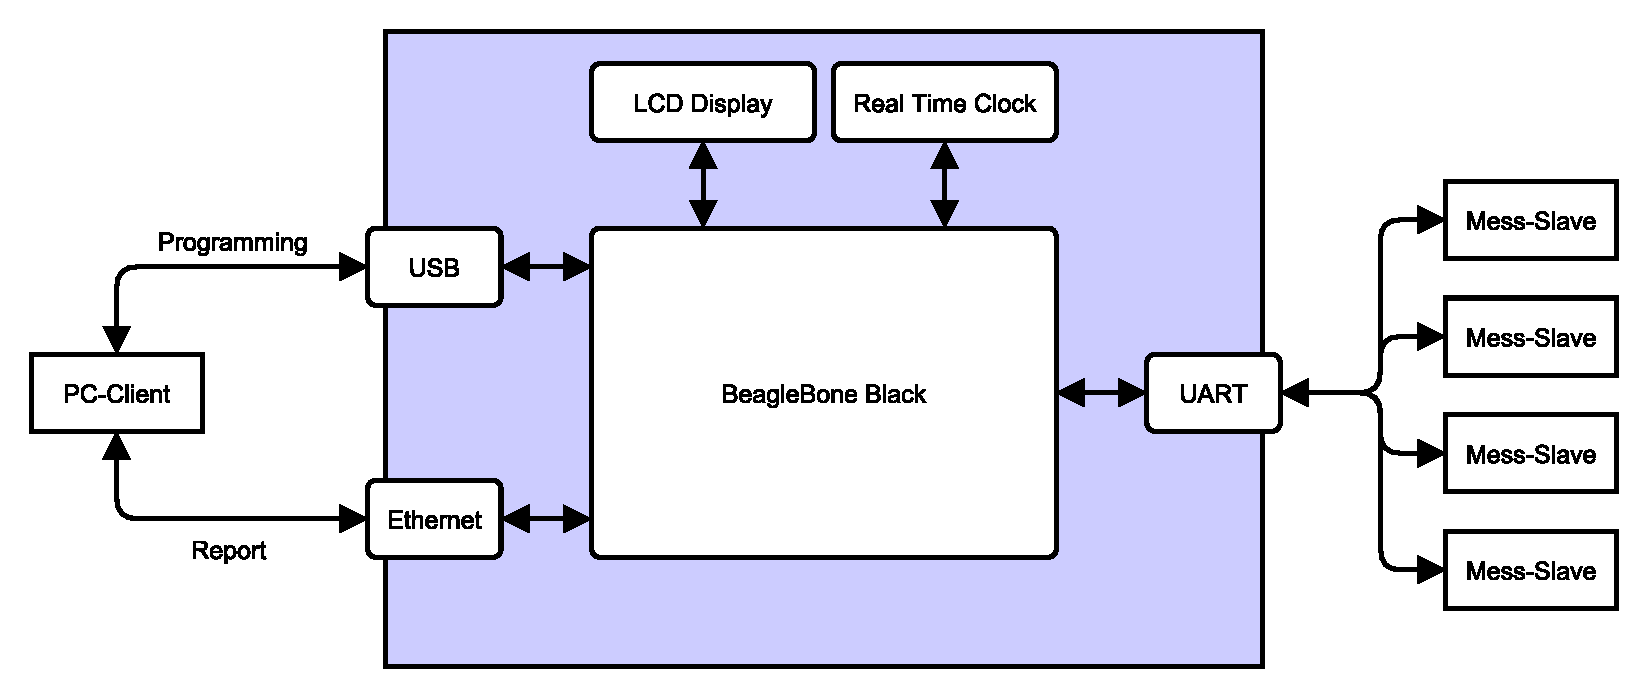
\includegraphics[width=0.8\textwidth ]{img/general/UebersichtMaster.pdf}
\caption{Übersicht Hardware}
\label{figure_AufbauBleagleBone}
\end{center}
\end{figure}

Das BeagleBone selbst ist bereits sehr Leistungsstark. Um jedoch weiter Funktionen und Schnittstellen hinzuzufügen, existieren Capes. Ein Cape ist eine für das BeagleBone konzipierte Erweiterung, die direkt auf das BeagleBone aufgesteckt werden kann. Die Treiber vieler dieser Capes sind bereits in dem Betriebssystem des BeagleBones integriert oder werden vom Hersteller bereitgestellt. Somit ist die Inbetriebnahme sehr komfortable.


\begin{figure}[H]
\minipage{0.30\textwidth}
  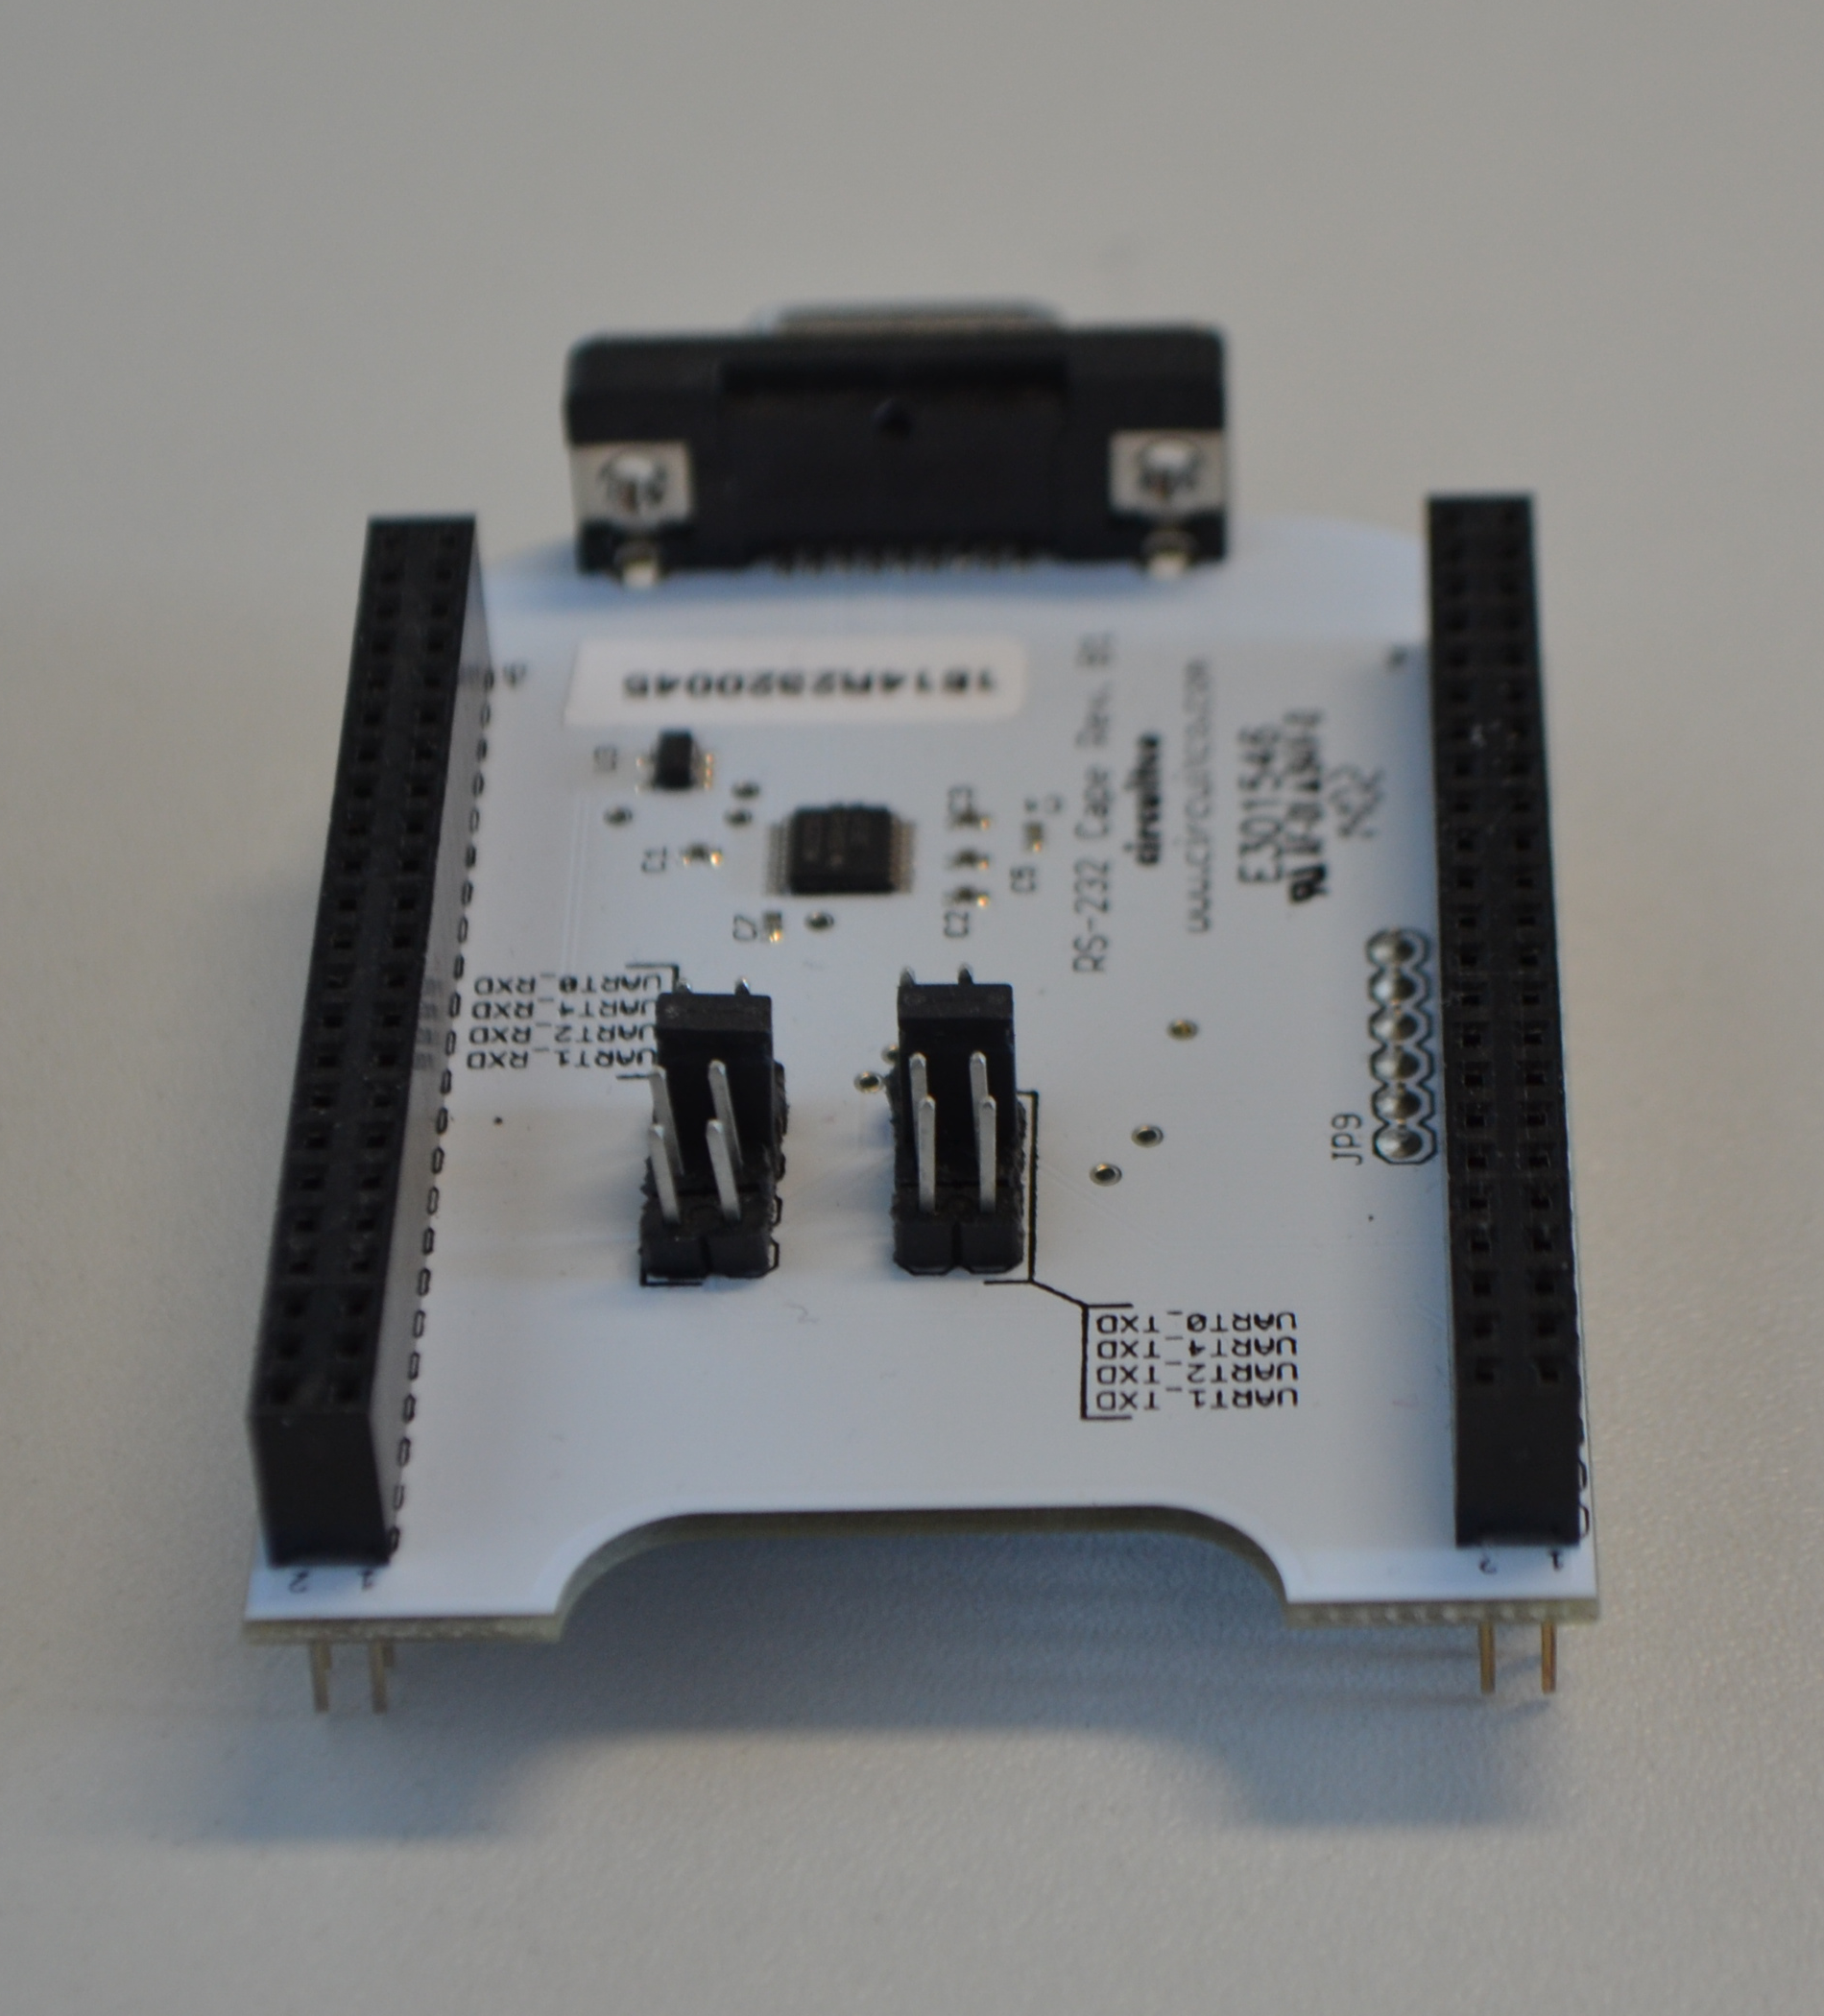
\includegraphics[width=\linewidth]{img/general/CapeRS232.png}
  \caption{RS232 Cape}\label{figure_CapeRS232}
\endminipage\hfill
\minipage{0.30\textwidth}
  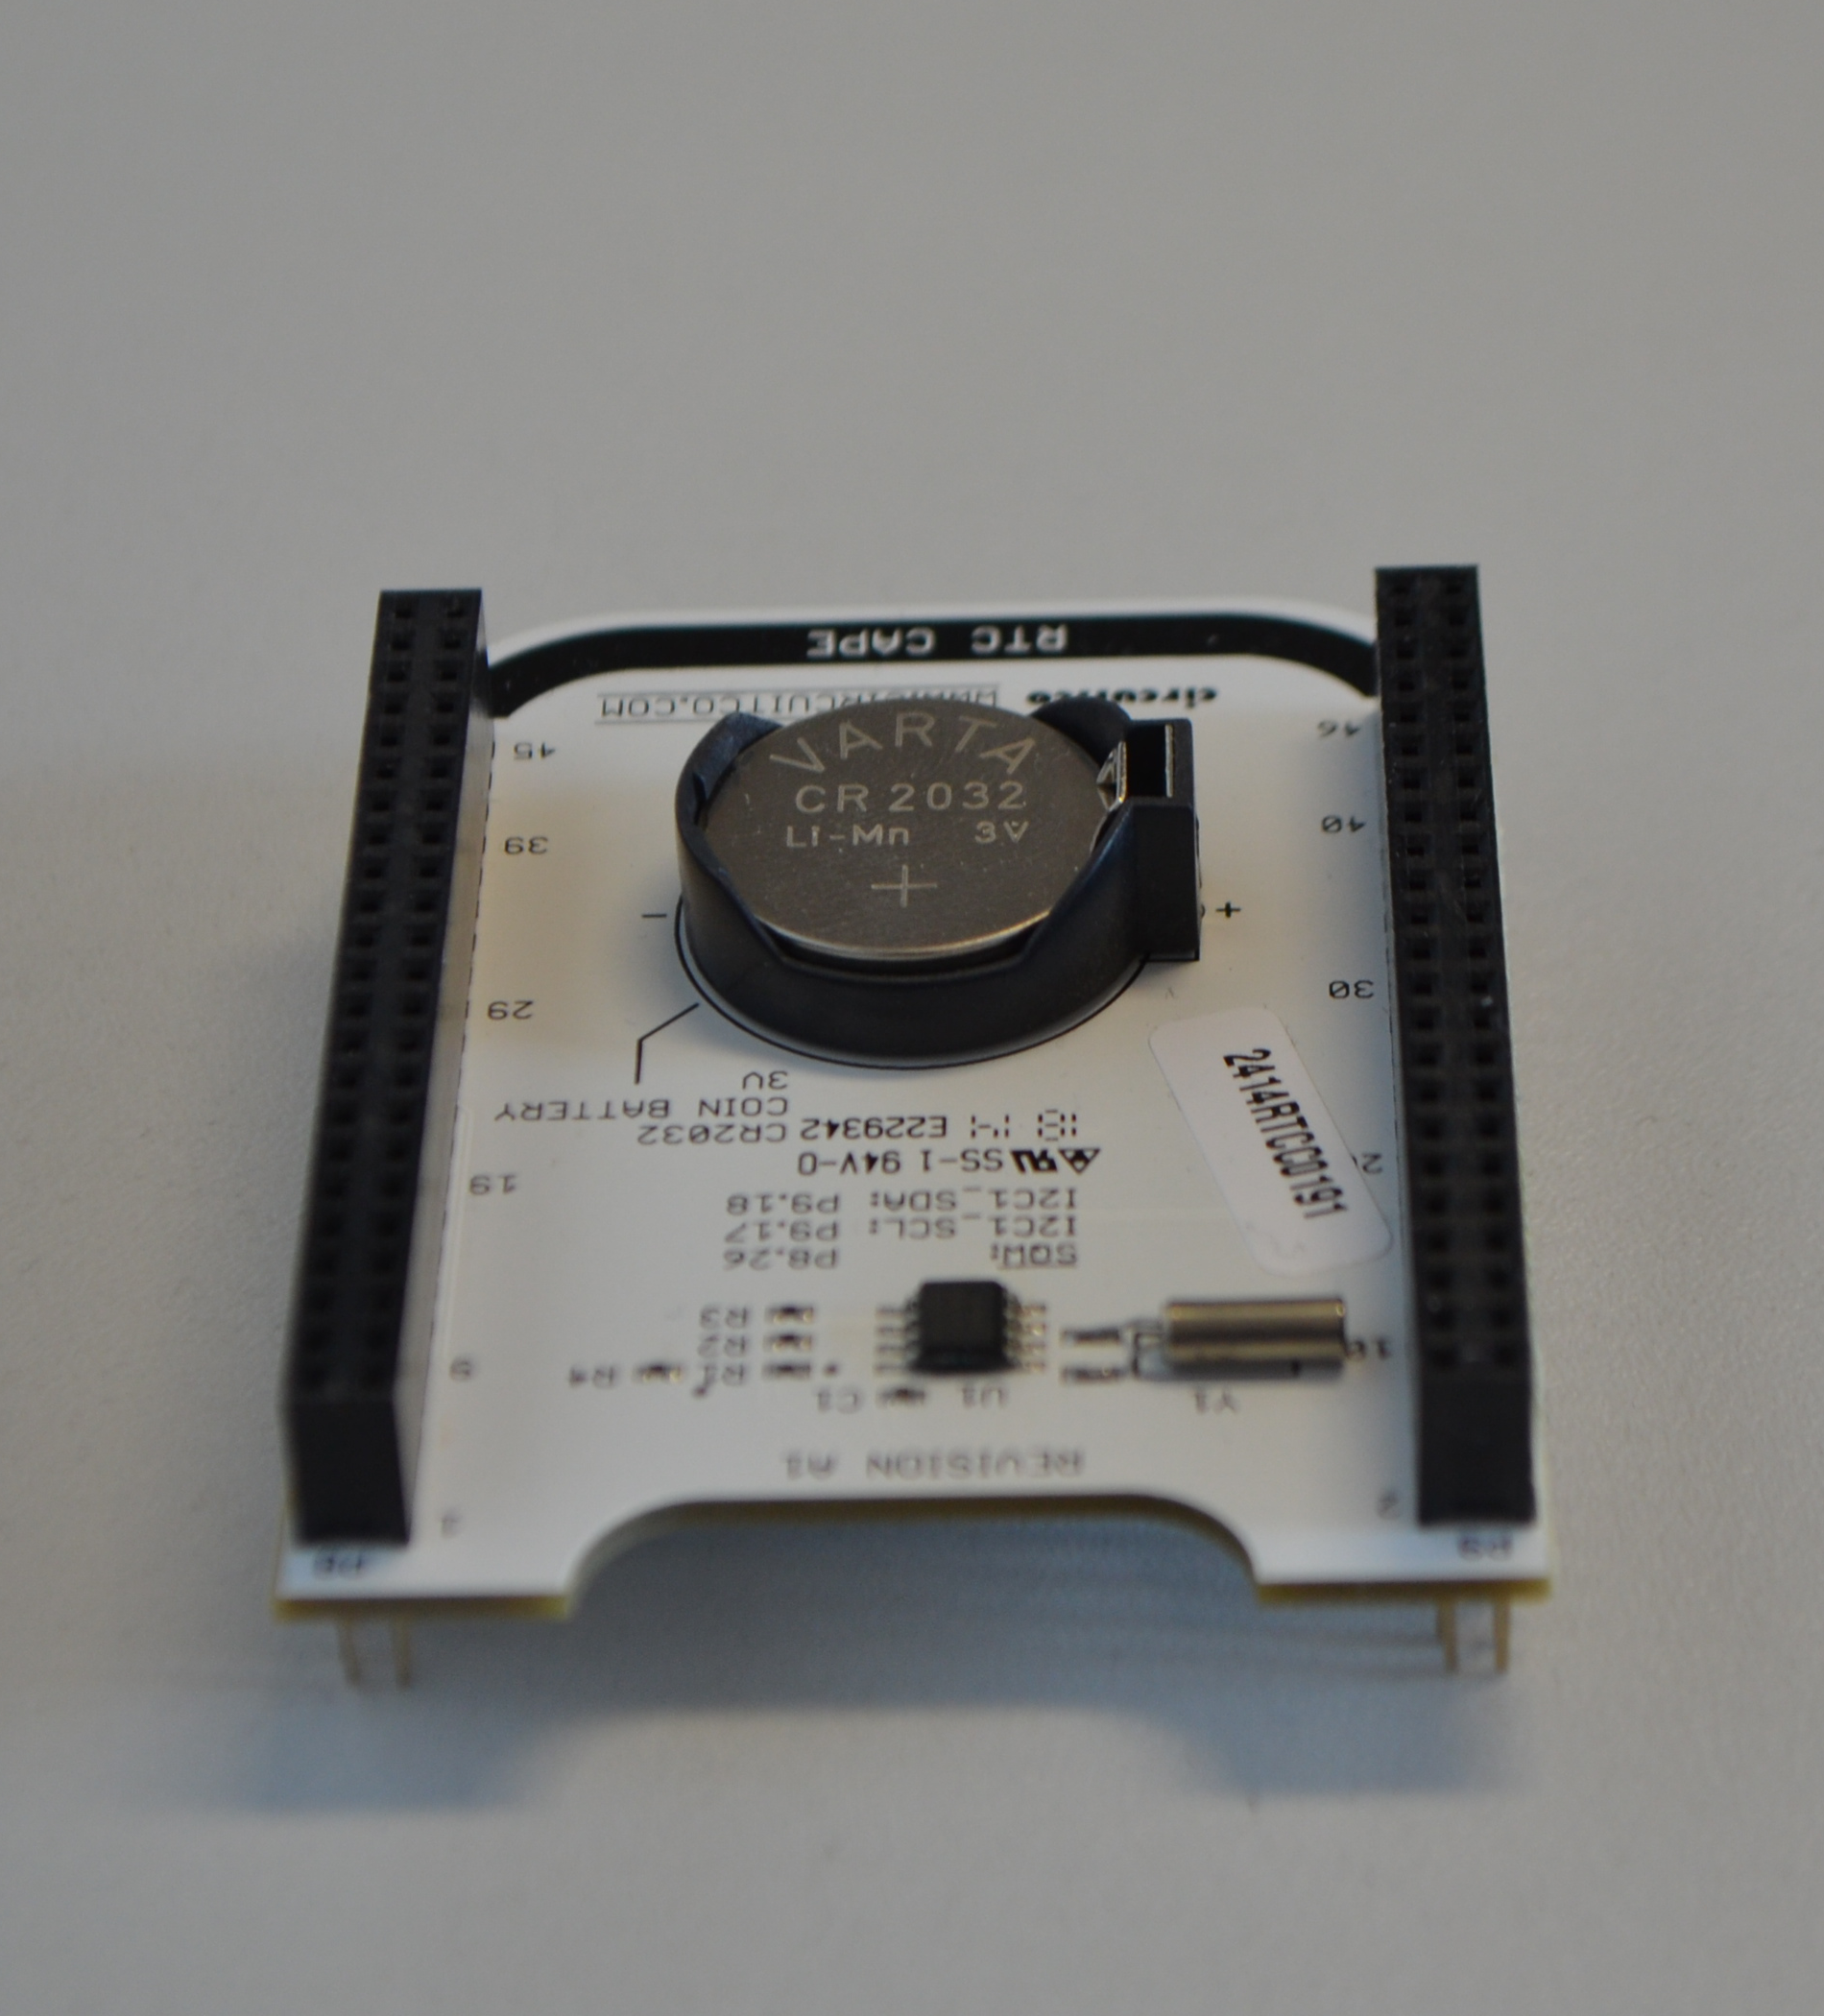
\includegraphics[width=\linewidth]{img/general/CapeRTC.png}
  \caption{RTC Cape}\label{figure_CapeRTC}
\endminipage\hfill
\minipage{0.30\textwidth}%
  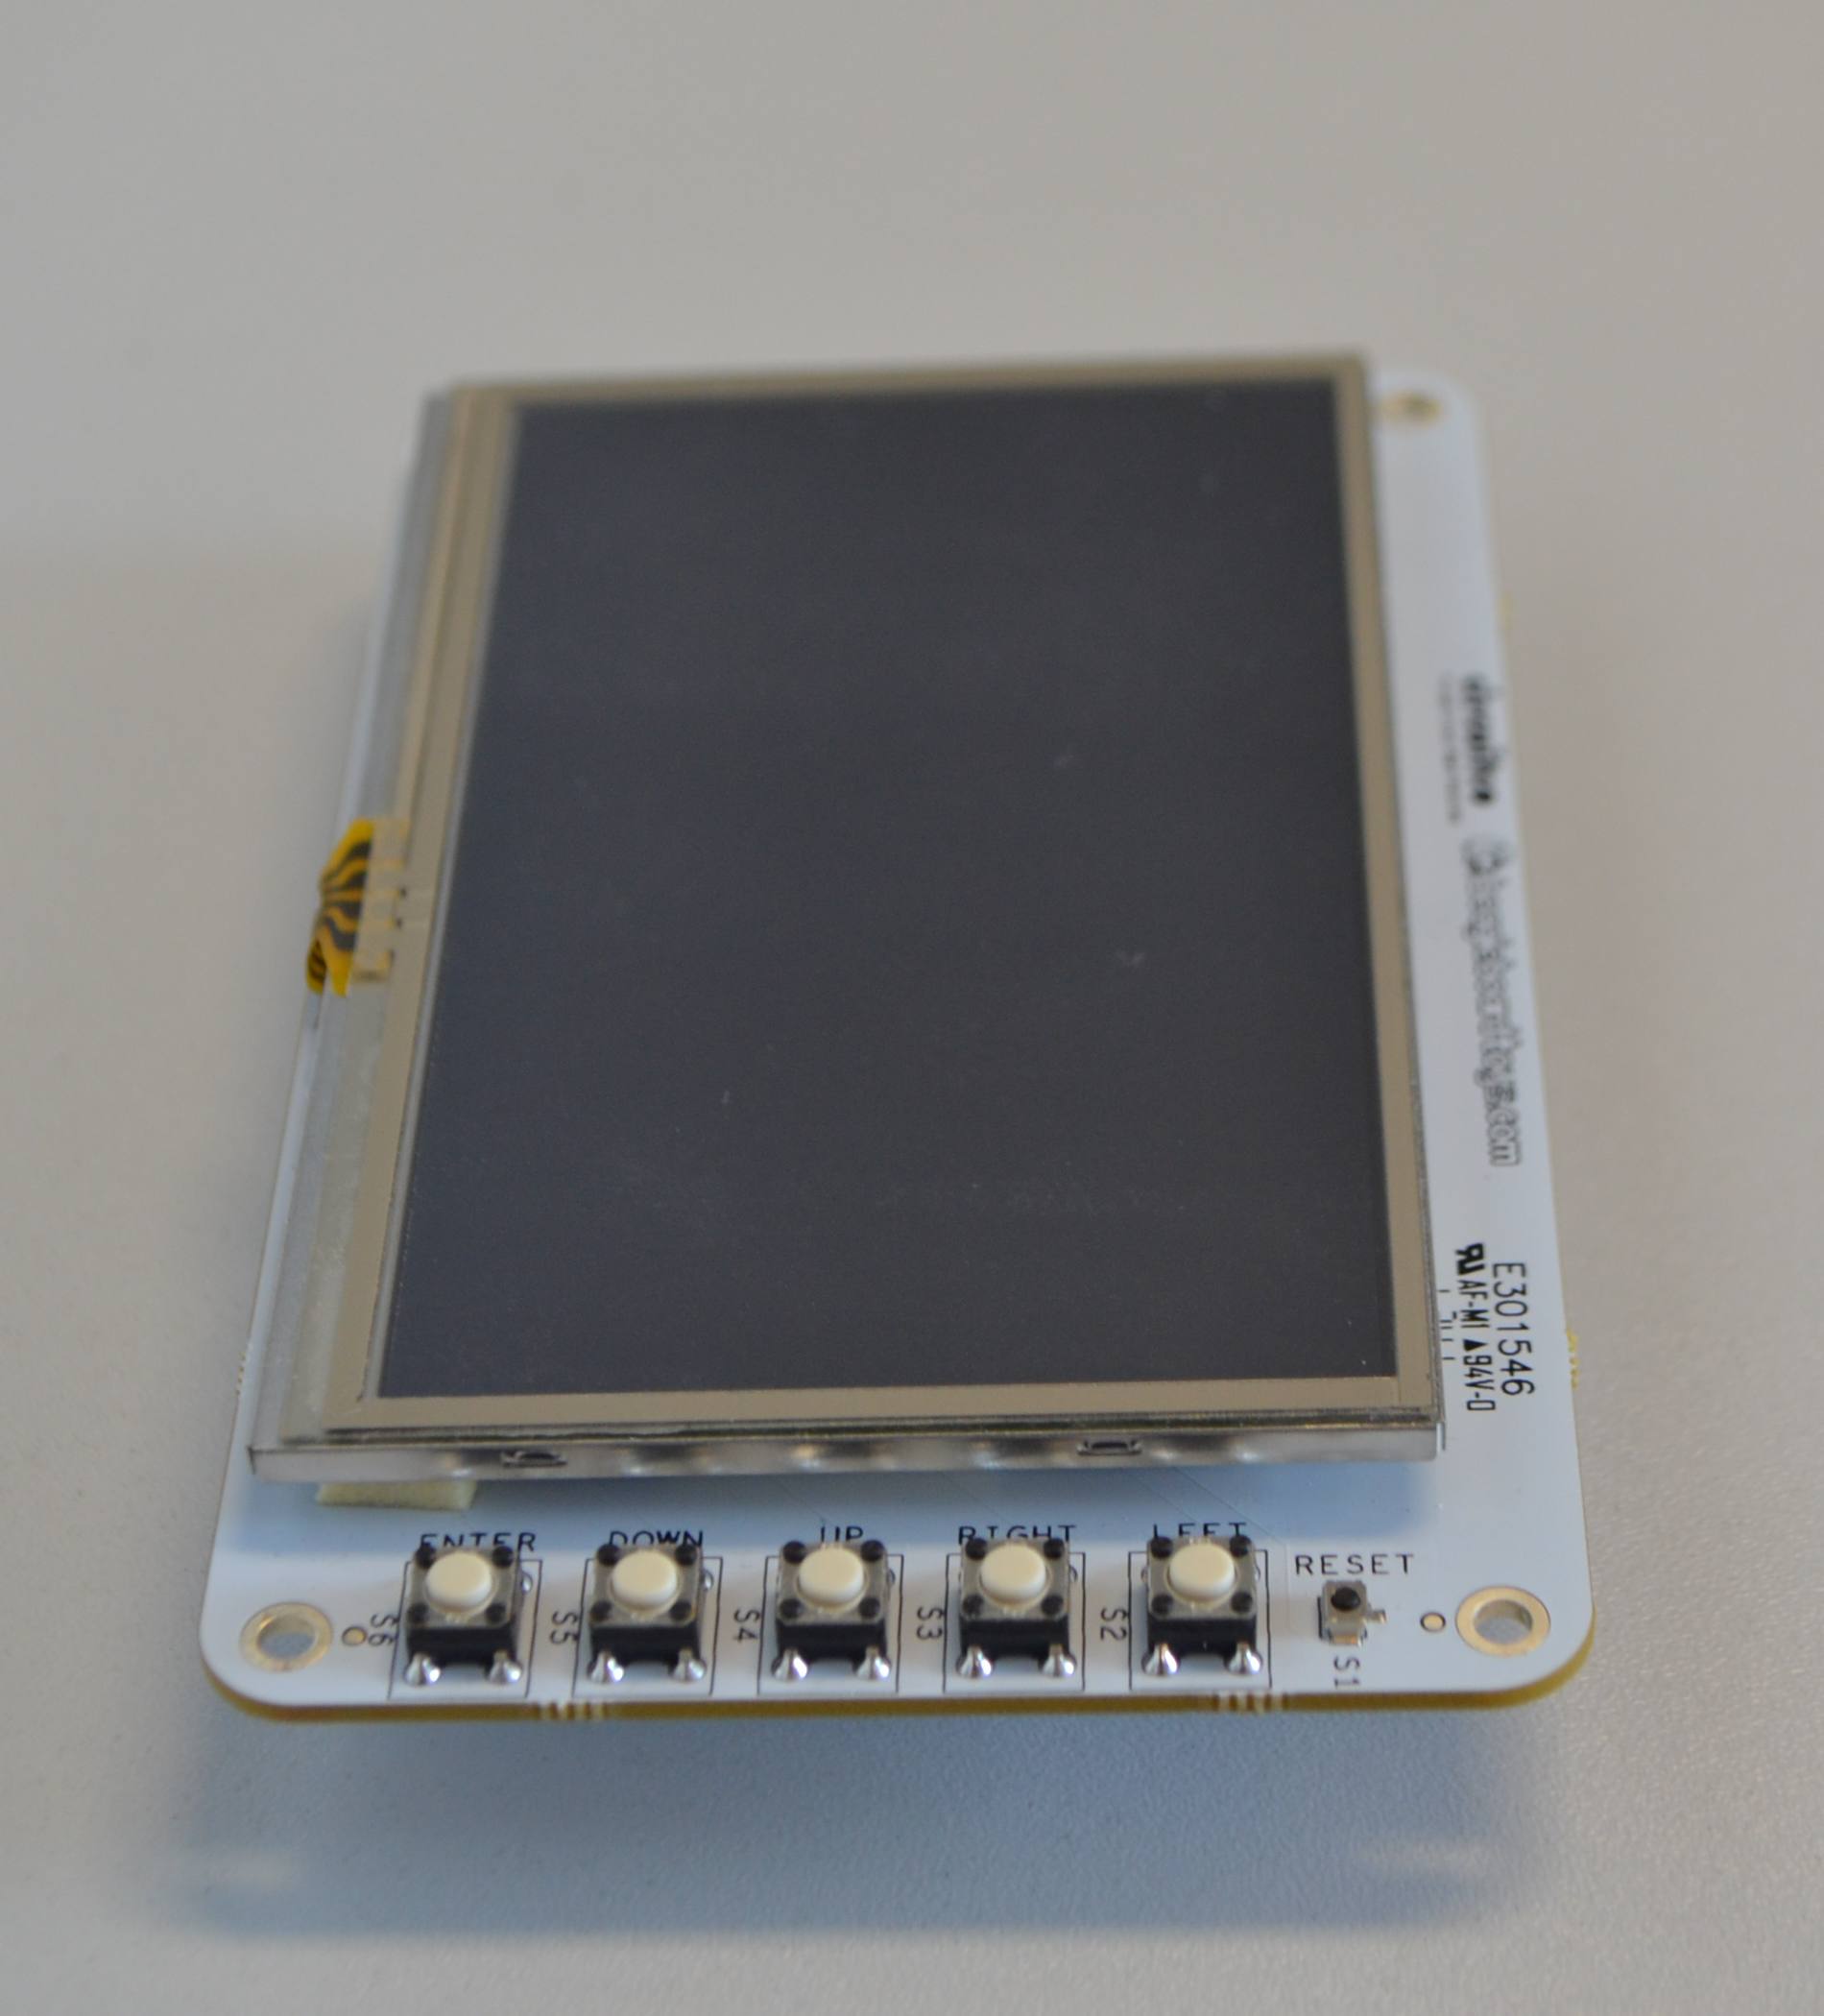
\includegraphics[width=\linewidth]{img/general/CapeLCD.png}
  \caption{LCD Cape}\label{figure_CapeLCD}
\endminipage
\end{figure}


Zur Kommunikation mit den Mess-Clients wird die \ac{UART} Schnittstelle des BeagleBone Black verwendet. Dafür wird ein RS232 Cape eingesetzt (siehe Abbildung \ref{figure_CapeRS232}). Das Cape führt die seriellen Ports UART0, UART1, UART2 und UART4 auf einen 9-poligen seriellen Stecker. Es bietet die Möglichkeit zwischen den verschiedenen Ports mittels eines Jumper auf dem Cape zu wechseln. Angeschlossen wird nach dem 3-wire Prinzip. Dabei werden lediglich Rx, Tx und die Masse verbunden. Somit ist keine Hardware-Flusssteuerung möglich.\ 

Da das BeagleBone Black kein eigenes \ac{RTC} Modul besitzt, wird auch dieses durch ein Cape hinzugefügt (siehe Abbildung \ref{figure_CapeRTC}). Es beinhaltet eine 3V Knopfbatterie um auch im Falle einer Stromunterbrechung die aktuelle Zeit nicht zu verlieren. Dies ist sehr wichtig, da es erforderlich ist, dass das BeagleBone die aktuelle Uhrzeit und das aktuelle Datum jederzeit kennt. Denn beim Erfassen der Messdaten wird ein Zeitstempel angelegt um die Daten später zeitlich zuordnen zu können. Sollte dieser Zeitstempel nicht korrekt sein, sind die Daten bei der Auswertung nicht gültig.\ 

Um die Statusanzeige detailliert darstellen zu können, wird ein resistives LCD-Touchscreen Display eingesetzt. Es hat eine Größe von 4,3 Zoll bei einer Auflösung von 480x272 Pixeln. Dabei handelt es sich ebenso um ein Cape (siehe Abbildung \ref{figure_CapeLCD}) . Dadurch ist es möglich, das BeagleBone Black trotz den Erweiterungen kompakt zu halten. Denn die Capes sind untereinander stapelbar (siehe Abbildung \ref{figure_GestapelteCapes}).\ 


\begin{figure}[H]
\begin{center}
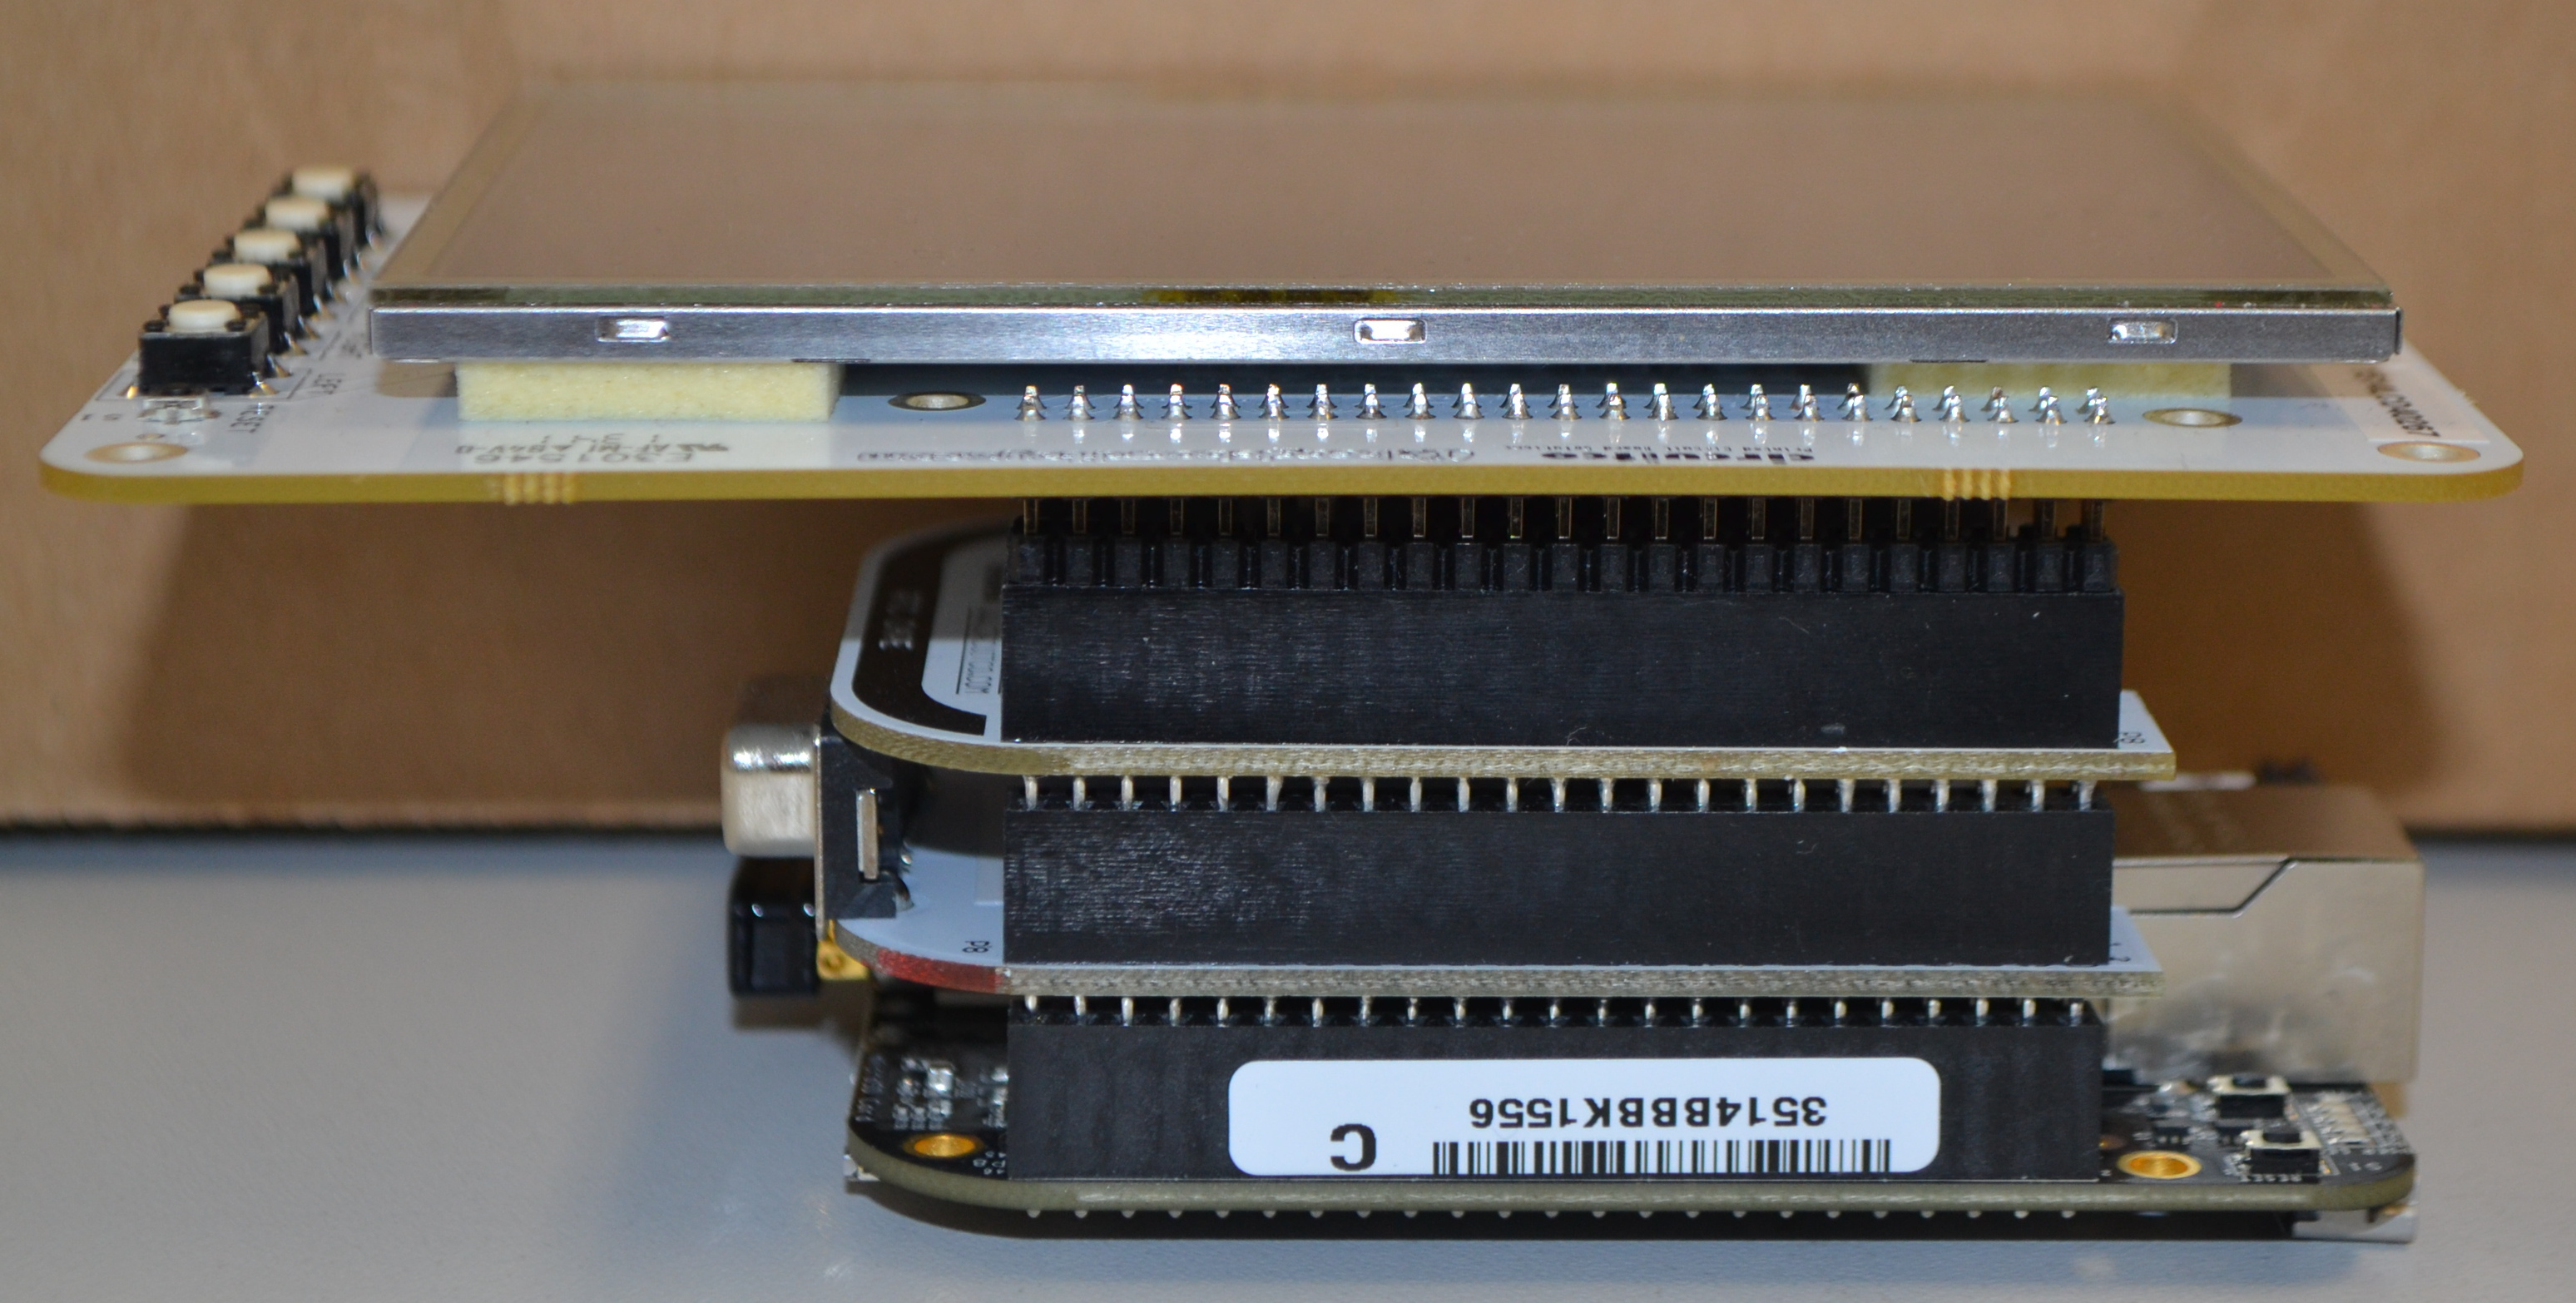
\includegraphics[width=0.5\textwidth ]{img/general/GestapelteCapes2.JPG}
\caption{Gestapelte Capes}
\label{figure_GestapelteCapes}
\end{center}
\end{figure}

Die USB Schnittstelle, welche zur Programmierung des BeagleBones verwendet wird, ist bereits vollständig einsatzbereit. Ebenso ist die Ethernet Schnittstelle, welche für den Fernzugriff auf das BeagleBone genutzt wird standardmäßig vollständig integriert.

\section{Software}
\label{ServerSoftware}

\begin{figure}[H]
\begin{center}
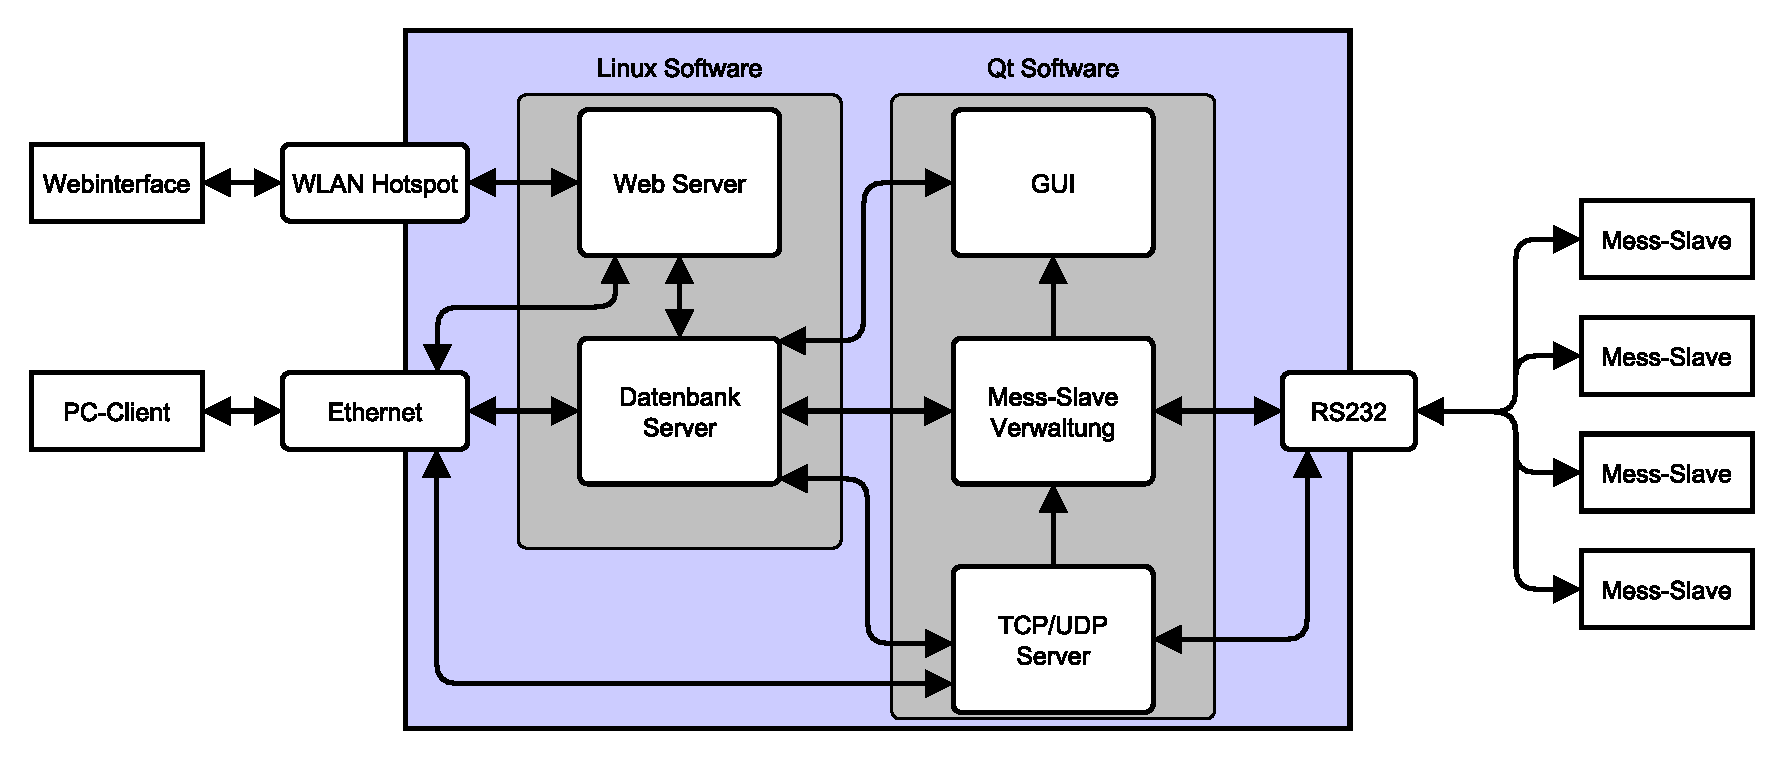
\includegraphics[width=0.8\textwidth ]{img/general/UebersichtMasterSoftware.pdf}
\caption{Übersicht Software}
\label{figure_GestapelteCapes}
\end{center}
\end{figure}

Das Software System setzt sich aus zwei Teilen zusammen. Zum Einen die selbst zu programmierende Software, welche in C++ unter Verwendung der Klassenbibliothek Qt (siehe Abschnitt \ref{section_Qt}) programmiert ist und zum Anderen die verschiedenen Softwarepakete die für das Linux Betriebssystem zur Verfügung stehen.\\
Im folgenden Abschnitt wird auf beide Softwareteile eingegangen. Zunächst werden die Bestandteile Mess-Client Verwaltung, Benutzeroberfläche und TCP/UDP-Server der Qt Anwendung näher erläutert und anschließend wird auf Datenbankserver, den Webserver und WLAN Hotspot eingegangen.

\subsection{Mess-Client Verwaltung}
\label{section_messclientverwaltung}
Die Verwaltung der Mess-Clients ist der Hauptprozess der Software. In diesem Programmteil wird die Kommunikation mit den Mess-Clients realisiert. Dabei sind die Grundaufgaben die Messdatenerfassung, das Erkennen von neuen Mess-Clients und die automatische Eingliederung dieser in das System.

\subsubsection{Mess-Client Anmeldung}

\begin{figure}[H]
\begin{center}
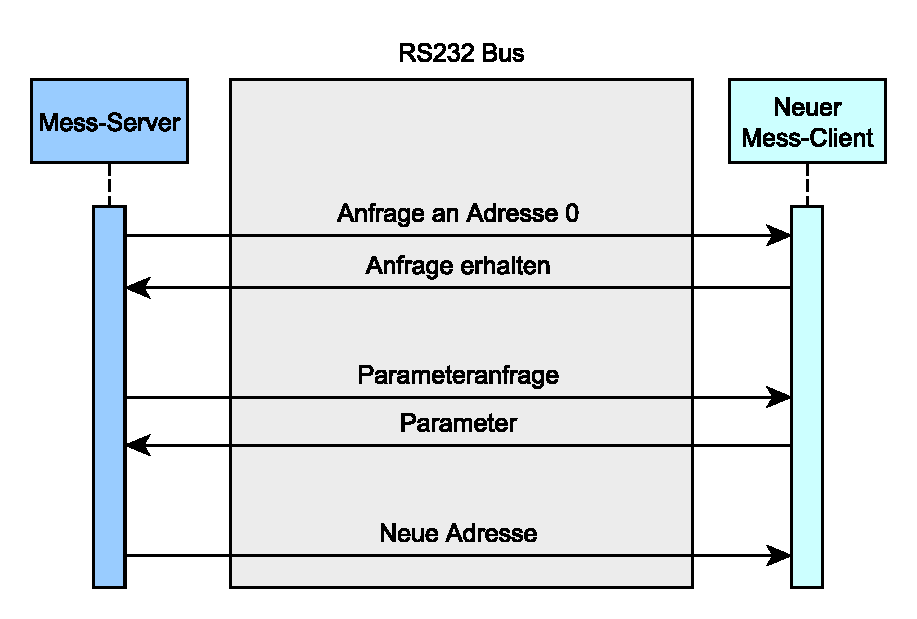
\includegraphics[width=0.6\textwidth ]{img/general/MessClientAnmeldung.pdf}
\caption{Mess-Client Anmeldung}
\label{figure_MessClientAnmeldung}
\end{center}
\end{figure}
 
 
Um in das bestehende System eingegliedert zu werden, muss jeder Mess-Client sich bei dem Mess-Server anmelden (siehe Abbildung \ref{figure_MessClientAnmeldung}). Dafür hat jeder neue Mess-Client die RS232 Adresse 0. Der Mess-Server überprüft in regelmäßigen Abständen, ob über die Adresse 0 ein Mess-Client erreichbar ist. Sobald dies der Fall ist, übermittelt der entsprechende Mess-Client seine Parametrierung an den Mess-Server. Die Parameter werden dann automatisch vom Mess-Server in der Datenbank abgelegt. Im Anschluss bekommt der Mess-Client eine neue Adresse zugewiesen über die er in Zukunft im System erreichbar ist.


 
\subsubsection{Messdatenerfassung}

Der Hauptzyklus der Software ruft kontinuierlich die Messdaten von den Mess-Clients ab. Dafür wird ständig geprüft ob Messungen erforderlich sind. Dies geschieht durch den Vergleich der vergangenen Zeit zur letzten Messung und den gegebenen Parametern für die Messintervalle. In der Tabelle \ref{table_ParameterMessintervalle} finden sich diese Parameter.\\


\begin{table}[H]
\begin{center}
\begin{tabular}{|l|l|}\hline
Parameter & Beschreibung \\ \hline
duration\_int1 & Dauer des 1. Zeitraums\\  \hline
duration\_int2 & Dauer des 2. Zeitraums\\  \hline
interval\_1 & Abstand zwischen den Messungen im 1. Zeitraum\\  \hline
interval\_2 & Abstand zwischen den Messungen im 2. Zeitraum\\  \hline
interval\_3 & Abstand zwischen den Messungen nach dem 2. Zeitraum\\ \hline
\end{tabular}
\caption{Parameter der Messintervalle}
\label{table_ParameterMessintervalle}
\end{center}
\end{table}


Ob eine Messung erforderlich ist, lässt sich aus den gegebenen Parametern ableiten. So wird zuerst geprüft, welcher Zeitraum (\textit{duration\_int1-2}) derzeit zutrifft. Dazu wird die vergangene Zeit seit der ersten Messung mit dem Zeitraum abgeglichen. Sollten noch keine Ergebnisse vorhanden sein, ergibt dies die Erforderlichkeit einer Messung. Wenn der passende Zeitraum ausgemacht ist, wird das dazugehörige Intervall zwischen den einzelnen Messungen (\textit{interval\_1-3}) ausgemacht. Dann wird geprüft, ob die vergangene Zeit seit der letzten Messung größer ist als dieses Intervall.\ 

Anschließend wird geprüft ob der Mess-Client verfügbar ist. Dazu wird eine Namensanfrage über die RS232 Schnittstelle verschickt. Bei einer positiven Antwort wird dann eine Messung durchgeführt. Dabei werden alle \acp{ADC} der 64 möglichen \acp{DUT} mittels \textit{ADC-Value}-Befehls (siehe Tabelle \ref{table_RS232Commands}) ausgelesen. Sobald alle 64 Werte erfolgreich ermittelt sind, werden sie in der Datenbank abgelegt. \\
Sollte keine Antwort auf die Namensanfrage erfolgen, wird in den nächsten Zyklen erneut versucht eine Verbindung zu etablieren. Bei kontinuierlich erfolglosen Verbindungsversuchen, informiert das System den Nutzer nach einer festgelegten Zeit der Abwesenheit über die Unerreichbarkeit.
 

 
\newpage
\subsection{Benutzeroberfläche}
Um die Anforderung der Statusüberwachnung zu erfüllen, verfügt das BeagleBone über eine \ac{GUI}. Sie soll einen einfachen Überblick über die aktuellen Vorgänge bieten und auf einen Blick den Status des Mess-Servers wiedergeben.\\

Status abhängig von freiem Disk Space, Boards erreichbar oder nicht, TCP Server


\newpage
\subsection{TCP/UDP Server}
\label{section_TCPUDPServer}
Um auf Netzwerkanfragen reagieren zu können, ist sowohl ein UDP-Server für Broadcast-Nachrichten als auch ein TCP-Server für die direkte Kommunikation realisiert.\\
Der UDP-Server dient dabei zur dynamischen Erkennung im Netzwerk. Dabei antwortet der Mess-Server auf Broadcast-Nachrichten mit seiner IP-Adresse und seinem Namen. Dies ermöglicht die einfache Eingliederung der Mess-Server in ein Netzwerk.
Der TCP-Server nimmt RS232- und SQL-Befehle an und leitet diese weiter. Dies ermöglicht den Fernzugriff auf die einzelnen Mess-Clients über ein Netzwerk.\\

\begin{table}[H]
\begin{center}
\begin{tabularx}{\textwidth}{|c|c|c|X|}\hline 
 Befehl & Typ & Daten & Kommentar \\ \hline
 BeagleSendYourIP & UDP & - & Das BeagleBone antwortet dem Sender mit seiner IP Adresse und seinem Namen  \\ \hline
 BeagleUpdateConfig & UDP & - & Das BeagleBone aktualisiert seine Konfiguration aus der Config-Datei \\ \hline
 RS232CMD: & TCP & Nachricht & Das BeagleBone sende den empfangenen Rahmen über seine RS232 Schnittstelle \\ \hline
\end{tabularx}
\caption{Ethernet Befehlsliste}
\label{table_EthernetCommands}
\end{center}
\end{table}

Der TCP/UDP-Server ist vor allem für die Kommunikation mit dem PC-Client zuständig. Um Mess-Server im Netzwerk zu finden, wird von ihm ein \textit{BeagleSendYourIP} Befehl als Broadcast-Nachricht versendet. Sollte ein Mess-Server diese Nachricht empfangen, antwortet er an die Sendeadresse mit der eigenen IP Adresse und dem eigenen Namen.\ 

Über den \textit{RS232CMD:} Befehl kann von einem PC-Client aus direkt mit einem am RS232 Bus angeschlossenen Mess-Client kommuniziert werden. der TCP-Server dient dabei als Tunnel für die Kommunikation (siehe Abbildung \ref{figure_RS232Tunnel}). Anfragen werden vom Mess-Server angenommen und weitergeleitet. Die Antworten nehmen den umgekehrten Weg zurück. Zur Sicherstellung der alleinigen Verwendung der RS232 Schnitstelle, pausiert der TCP-Server die anderen Prozesse, die auf die Schnittstelle zugreifen, für die Dauer der Kommunikation.\ 


\begin{figure}[H]
\begin{center}
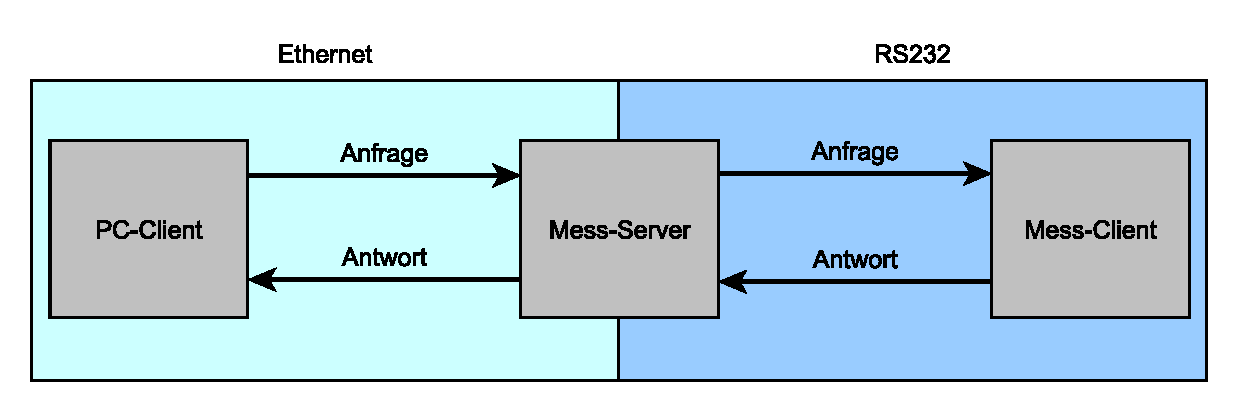
\includegraphics[width=0.7\textwidth ]{img/general/RS232Tunnel.pdf}
\caption{RS232 Tunnel}
\label{figure_RS232Tunnel}
\end{center}
\end{figure}

\newpage
\subsection{Web Server und WLAN Hotspot}
\label{section_WebServerWLANHotspot}

Mit Hilfe eines Web Servers ist es auch lokal möglich eine Übersicht über die gesammelten Daten auf dem Mess-Server zu erhalten. Als Schnittstelle steht ein WLAN Hotspot zur Verfügung.\ 

Als Webserver dient Lighttpd (auch: Lighty). Lighttpd ist laut \cite{bogus2008lighttpd} ein erweiterbarer, modularer, Single-Threaded, hoch hochperformanter Webserver, der selbst Apache oder Microsofts IIS in den meisten Einstellungen übertrifft. Besonders auf kleinen System mit begrenzten Ressourcen komme er häufig zum Einsatz. Trotzdem vertrauen auch große Webanbieter wie YouTube oder Wikipedia auf seine Effizienz.\\
Zusätzlich sind das PHP und MySQL \ac{CGI} Modul installiert um die Messergebnisse aus der Datenbank dynamisch darstellen zu können. 

Der Webserver ist sowohl über die normale Ethernet Verbindung als auch einen WLAN Hotspot erreichbar. Für die Realisierung des WLAN Hotspots wird ein EDIMAX EW-7811Un WLAN Dongle über den Host-USB Port des BeagleBone Black betrieben.\\
Als Hotspot Software dient Hostapd. Hostapd ist ein IEEE 802.11 Accesspoint und IEEE 802.1X/WPA/WPA2/EAP/RADIUS Authentificator (vgl. \cite{LinuxWireless}) und verwaltet die Zugriffe auf den Hotspot.\\
Zusätzlich müssen Geräten die sich über den Hotspot mit dem BeagleBone Black verbinden eine IP-Adresse zugewiesen werden. Dafür kommt der DNS- und DHCP-Server dnsmasq zum Einsatz.\\


\begin{figure}[H]
\begin{center}
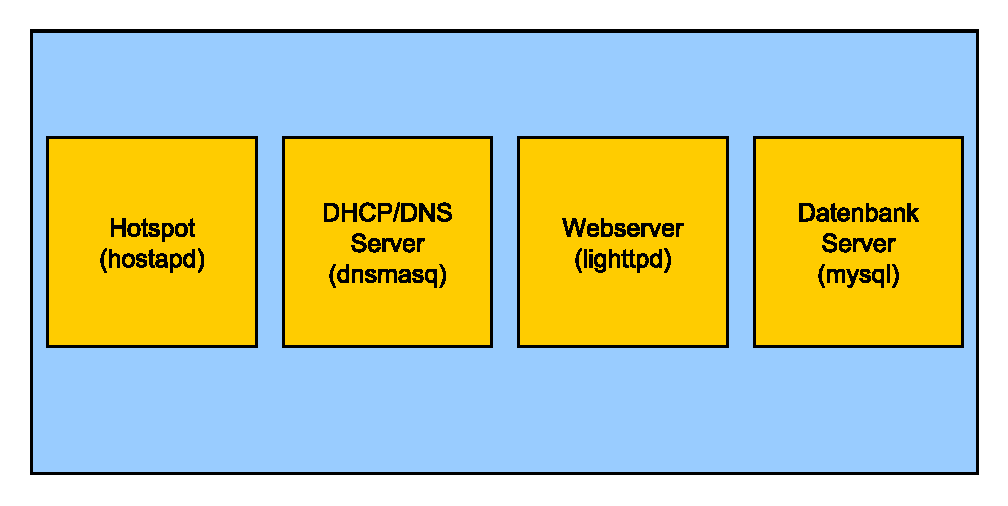
\includegraphics[width=0.8\textwidth]{img/general/WebinterfaceAufbau.pdf}
\caption{Webinterface Aufbau}
\label{ERM}
\end{center}
\end{figure}

\newpage
 
\subsection{Datenbank Server}
\label{section_EntwurfDatenbank}

Wie in vorangehenden Kapiteln bereits erwähnt, werden alle Messdaten und Betriebsparameter in einer MySQL-Daten abgelegt. Der MySQL-Datenbankserver läuft auf dem BeagleBone Black und ist über das Netzwerk erreichbar.

Aus den Anforderungen ergibt sich folgendes \ac{ERM} (siehe Abbildung \ref{ERM}). \\

\begin{figure}[H]
\begin{center}
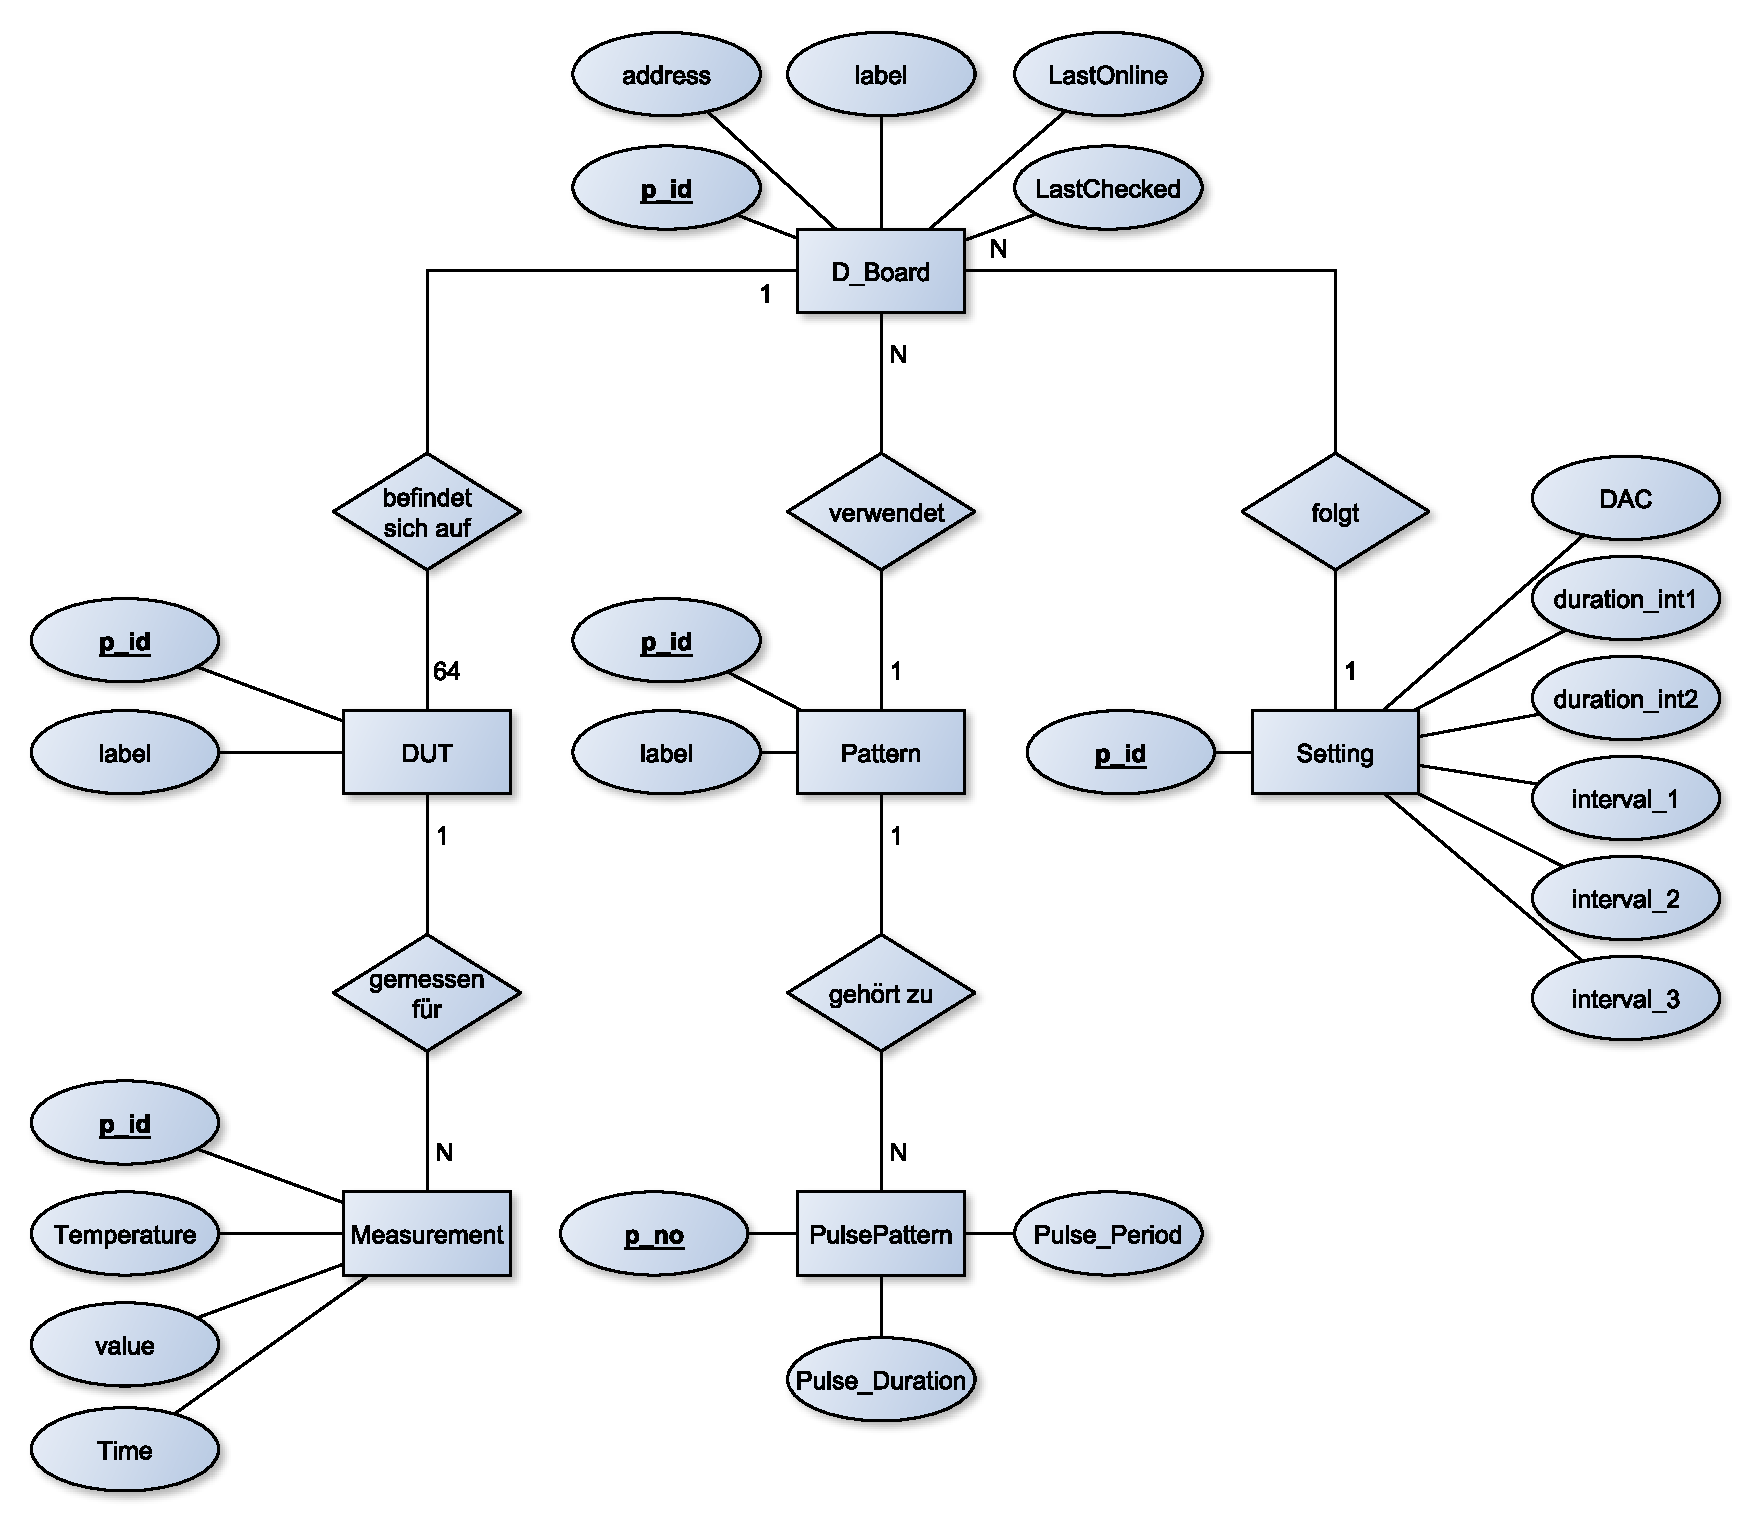
\includegraphics[width=0.9\textwidth]{img/general/ER_Diagramm.pdf}
\caption{Entity Relationship Modell}
\label{ERM}
\end{center}
\end{figure}

\subsubsection{Tabellen}
Im folgenden Abschnitt wird näher auf die einzelnen Tabellen und ihre Beziehungen untereinander eingegangen. Außerdem werden die Attribute näher erläutert.

\newpage
\textbf{Tabelle D\_Board}\\

\begin{table}[H]
\begin{center}
\begin{tabular}{|l|l|}\hline
Parameter & Datentyp \\ \hline
p\_id & INTEGER PRIMARY KEY\\ 
address & INTEGER UNIQUE\\ 
label & VARCHAR(255) UNIQUE\\ 
LastOnline & TIMESTAMP\\ 
LastChecked & TIMESTAMP\\ 
f\_settingid & INTEGER FOREIGN KEY\\
f\_Patternid & INTEGER FOREIGN KEY\\ \hline
\end{tabular}
\caption{Tabelle D\_Board}
\label{table_TabelleD_Board}
\end{center}
\end{table}


Die Tabelle D\_Board (steht für Degradations-Board) speichert alle im System registrierten Mess-Clients. Jeder Mess-Client hat eine einzigartige Identifikationsnummer (\textit{p\_id}), welche gleichzeitig den Primärschlüssel (englisch: primary key) repräsentiert. Um die Mess-Clients später leserlich auseinanderhalten zu können, verfügen sie zusätzlich über einen Namen (\textit{label}), der einzigartig sein muss.\\
Zur Kommunikation wird jedem Board eine einzigartige Adresse (\textit{address}) zugeordnet. Boards die eine Adresse haben, werden als aktive Boards bezeichnet. Es kann davon ausgegangen werden, dass sie innerhalb des Systems erreichbar sind. Außerdem ist auch möglich, dass ein Board keine Adresse hat. In diesem Fall ist das Board als inaktiv anzusehen. Die Daten sind zwar noch in der Datenbank, jedoch ist es nicht mehr erreichbar und es werden keine neuen Messwerte aufgenommen. Diese Inaktivität entsteht, wenn ein Board für eine zu lange Zeit nicht Erreichbar ist. Denn in einem solchen Fall, wird die Adresse aufgrund des beschränkten Adressraumes freigegeben.\\
Jedes Degradationsboard besitzt einen Zeitstempel (\textit{LastOnline}) für den Zeitpunkt der letzten erfolgreichen Kontaktaufnahme. Diese Information ist notwendig um die Dauer der Abwesenheit ermitteln und den Nutzer dahingehen in Kenntnis setzen zu können.\\
Des Weiteren gibt es noch einen Zeitstempel (\textit{LastChecked}) für den letzten Zeitpunkt des Versuches einer Kontaktaufnahme, welcher notwendig ist, um unnötig häufige Kontaktversuche zu vermeiden. So soll ein Degradationsboard nicht häufiger als alle 10 Minuten kontaktiert werden um die Performance zu erhöhen.\\
Zusätzlich folgt jedes Board genau einer Einstellung (Tabelle Setting). Diese Relation wird durch einen Fremdschlüssel (englisch: foreign key) mit der Identifikationsnummer einer Einstellung (\textit{f\_Settingid}) referenziert.\\
Außerdem hat jedes Board ein PulsePattern (Tabelle Pattern) zur Ansteuerung der Prüfobjekte. Dieses wird durch die Identifikationsnummer eines Patterns(\textit{f\_Patternid}) angegeben.


\newpage

\textbf{Tabelle Setting}\\

\begin{table}[H]
\begin{center}
\begin{tabular}{|l|l|}\hline
Parameter & Datentyp \\ \hline
p\_id & INTEGER PRIMARY KEY\\ 
DAC & INTEGER\\ 
duration\_int1 & INTEGER\\ 
duration\_int2 & INTEGER\\ 
interval\_1 & INTEGER\\ 
interval\_2 & INTEGER\\ 
interval\_3 & INTEGER\\ \hline
\end{tabular}
\caption{Tabelle Setting}
\label{table_TabelleSetting}
\end{center}
\end{table}

In der Tabelle Setting, werden die Einstellungen  für die verschiedenen Degradationsboards abgelegt. Jede Einstellung kann dabei mehreren Boards zugeordnet sein, wobei jedes Board nur eine Einstellung besitzt.\\
Der Primärschlüssel der Tabelle ist die Identifikationsnummer (\textit{p\_id}) jeder Einstellung. Als Nächstes gibt es die Vorverstärkung (\textit{DAC}) der Empfänger auf den Degradationsboards. Mithilfe der Vorverstärkung werden die gemessenen Signale der Prüfobjekte für die bessere Analyse durch den Analog-Digital-Konverter verstärkt. Darauf folgend kommen die Parameter zur Konfiguration der Messintervalle (siehe auch Tabelle \ref{table_ParameterMessintervalle}). Sie bestimmen die Zeiträume (\textit{duration\_int1 + 2}) und die Abstände zwischen den Messungen (\textit{interval\_1-3}) innerhalb dieser Zeiträume.\\

\textbf{Tabelle DUT}\\

\begin{table}[H]
\begin{center}
\begin{tabular}{|l|l|}\hline
Parameter & Datentyp \\ \hline
p\_id & INTEGER PRIMARY KEY\\ 
label & VARCHAR(255)\\ 
f\_Boardid & INTEGER FOREIGN KEY\\ \hline
\end{tabular}
\caption{Tabelle DUT}
\label{table_TabelleDUT}
\end{center}
\end{table}

Die Tabelle DUT nimmt die einzelnen Prüfobjekte (\acp{DUT}) auf. Jedes Prüfobjekt gehört fest zu einem Degradationsboard. Dies wird durch den Fremdschlüssel mit der Identifikationsnummer des zu gehörenden Boardes (\textit{f\_Boardid}) referenziert.Außerdem hat jedes Prüfobjekt eine eindeutige Identifikationsnummer (\textit{p\_id}) als Primärschlüssel. Des Weiteren verfügt es über eine Bezeichnung (\textit{label}), um sich von den anderen Prüfobjekten des selben Boardes zu unterscheiden.



\textbf{Tabelle Pattern}\\

\begin{table}[H]
\begin{center}
\begin{tabular}{|l|l|}\hline
Parameter & Datentyp \\ \hline
p\_id & INTEGER PRIMARY KEY\\ 
label & VARCHAR(255)\\ \hline
\end{tabular}
\caption{Tabelle Pattern}
\label{table_TabellePattern}
\end{center}
\end{table}

In der Pattern Tabelle sind die Muster für die Signale zur Ansteuerung der Prüfobjekte. Die Muster haben eine Identifikationsnummer (\textit{p\_id}) als Primärschlüssel und eine Bezeichnung (\textit{label}) für die Leserlichkeit. Die Tabelle fasst die Signale aus der PulsePattern Tabelle zusammen um einfacher referenziert werden zu können.\\

\textbf{Tabelle PulsePattern}\\

\begin{table}[H]
\begin{center}
\begin{tabular}{|l|l|}\hline
Parameter & Datentyp \\ \hline
pf\_Patternid & INTEGER PRIMARY KEY FOREIGN KEY\\ 
p\_no & INTEGER NOT NULL\\
Pulse\_Duration & INTEGER\\
Pulse\_Period & INTEGER\\ \hline
\end{tabular}
\caption{Tabelle PulsePattern}
\label{table_TabellePulsePattern}
\end{center}
\end{table}

Die Tabelle PulsePattern enthält die Signale für die Muster in Tabelle Pattern. Die Identifikationsnummer des Musters(\textit{pf\_Patternid}) und die Position im Muster (\textit{p\_no}) dienen zusammen als ein Primärschlüssel. Die Identifikationsnummer des Musters(\textit{pf\_Patternid})dient dabei gleichzeitig als Fremdschlüssel und referenziert ein Muster. Dadurch ist es möglich sowohl die Zugehörigkeit zu einem spezifischen Muster als auch die Position in ihm einzigartig zu bestimmen. Die Signaldauer (\textit{Pulse\_Duration}) beschreibt die Dauer des aktiven Pegels innerhalb des Signals, während die Signalperiode (\textit{Pulse\_Period}) die Periodendauer des Signals angibt. So ergibt sich ein High-Pegel für die Dauer von $Pulse\_Duration$ und ein Low-Pegel für die Dauer von $Pulse\_Period - Pulse\_Duration$.\\

\newpage

\textbf{Tabelle Measurement}\\

\begin{table}[H]
\begin{center}
\begin{tabular}{|l|l|}\hline
Parameter & Datentyp \\ \hline
p\_id & INTEGER PRIMARY KEY \\ 
Temperatur & INTEGER\\
value & INTEGER\\
Time & TIMESTAMP DEFAULT CURRENT\_TIMESTAMP\\ \hline
\end{tabular}
\caption{Tabelle Measurement}
\label{table_TabelleMeasurement}
\end{center}
\end{table}

In der Measurement Tabelle werden die Messwerte der einzelnen Prüfobjekte gespeichert. Der Primärschlüssel ist auch hier die Identifikationsnummer (\textit{p\_id}). Zu jedem Messeintrag gehört die aktuelle Temperatur (\textit{Temperatur}), der gelesene Messwert (\textit{value}) und die aktuelle Zeit (\textit{Time}).




